\documentclass{article}
\usepackage[utf8]{inputenc}
\usepackage{geometry}
\usepackage{amsmath}
\usepackage{amssymb}
\usepackage{amsfonts}
\usepackage{graphicx}

\geometry{a4paper,
 total={170mm,257mm},
 left=15mm,
 right=15mm,
 top=10mm,}

\title{Cahier de kholle}

\begin{document}

\begin{center}
  \hrule
	\vspace{.4cm}
	{\textbf{\large cahier de kholle}}
\end{center}

{\textbf{Nom:}\ Arnaud Lelièvre \hspace{\fill} \vspace{0.5cm}}
{\textbf{}\  \hspace{\fill} \vspace{0.5cm}}
{\textbf{classe: MPSI 1}\ \hspace{\fill}}
\hrule
\date{}

\vspace{1cm}

\begin{center}
\textbf{\large Cahier de kholle de l'année de sup à Pasteur en MPSI 1}
\end{center} \vspace{0.2cm}

\begin{center}
\textbf{\large Mathématiques}
\end{center} \vspace{0.2cm}

\section{Kholle 1}
\subsection{kholleur/euse: M.Chen}

note: 17/20 \\
chapitre: Logique, ensembles, calcul algébrique\\

\subsection{question compliquée: Cauchy-Schwarz (mais vu en DM)}

\vspace{5mm}

\begin{equation}
  \left(\sum_{i=1}^{n} u_i v_i \right)^2 \leqslant \left(\sum_{i=1}^{n} u_i\right)^2 \left(\sum_{i=1}^{n} v_i \right)^2
\end{equation}

\textbf{\large résolution:}
\vspace{5mm}

\( \text{Posons } P(x) = \sum_{i=1}^n (u_i+xv_i)^2 \) \\
\( \sum_{i=1}^n u_i^2 + 2xu_i v_i +x^2 v_i^2 \) \hspace{5mm} \( \rightarrow \) \hspace{5mm} On reconnait un polynome du second degré en $x$ \\
$\rightarrow$ \hspace{2mm} On calcule son discriminant $\Delta = 4 \left( \left(\sum_{i=1}^n u_i v_i \right)^2 - \left(\sum_{i=1}^n v_i^2 \right) \left(\sum_{i=1}^n v_i^2 \right) \right)$ \hspace{5mm} \\
$\rightarrow$ \hspace{2mm} or $P(x) \geqslant 0$ car c'est la somme de termes au carré, donc $\Delta \leqslant 0$ \\
d'où \hspace{2mm} $\left( \left(\sum_{i=1}^n u_i v_i \right)^2 - \left(\sum_{i=1}^n v_i^2 \right) \left(\sum_{i=1}^n v_i^2 \right) \right) \leqslant 0$ \hspace{2mm} donc \hspace{2mm} $\left(\sum_{i=1}^{n} u_i v_i \right)^2 \leqslant \left(\sum_{i=1}^{n} u_i\right)^2 \left(\sum_{i=1}^{n} v_i \right)^2$


\subsection{kholleur/euse: M.De Laboulaye}

note: 14/20 \\
chapitre: Logique, calcul algébrique, sommes et produits, systèmes linéaires trigonométrie, complexes\\

\vspace{5mm}

problèmes compliqués, je n'aurais surement pas réussi sans les astuces qui m'ont été données

\subsection{kholleur/euse: M.Thai}

note: 11/20 \\
chapitre: Logique, calcul algébrique, sommes et produits, systèmes linéaires trigonométrie, complexes\\

\subsection{question raté (mais car j'ai paniqué, j'aurais due savoir directement)}

\vspace{0.5cm}

Démontrer que n'importe quelle fonction peut se décomposer en la somme d'une fonction paire et impaire \\ \\

\textbf{\large{résolution:}}

\vspace{5mm}

\underline{\textbf{Analyse:}} supposons que $ \forall x \in \mathbb{R}$ $f(x) = P(x) + I(x) $ avec $ P(x) $ une fonction paire et $I(x)$ une fonction impaire \\ \\
On a donc $\forall x \in \mathbb{R}:$ \\

$f(-x) = P(x) - I(x)$

et $f(x) = P(x) + I(x)$ \\ \\
donc en additionnant les lignes: \\

$P(x) = \frac{f(-x) + f(x)}{2}$

$I(x) = \frac{f(x) - f(-x)}{2}$

\vspace{5mm}
\underline{\textbf{Synthèse:}}\\ \\
$\frac{f(x) + f(-x)}{2} + \frac{f(x) - f(-x)}{2} = f(x)$


\subsection{kholleur/euse: M.Laillet}

note: 13/20 \\
chapitre: calcul différentielle et intégral, et fonctions usuelles

\subsection{question que j'aurais pu mieux faire: faire le graphe de la fonction W de Lambert}

Faire le graphe de l'application $\mathbb{W}$ tq $ \mathbb{W} \in \mathbb{R}^{\mathbb{R^{+}}}$ et $\forall x \in \mathbb{R^{+}} \mathbb{W}(x)e^{\mathbb{W}(x)} = \mathbb{I}_d(\mathbb{R^{+}})$

On a $\forall x \in \mathbb{R}^+ \mathbb{R^{+}} \mathbb{W}(x)e^{\mathbb{W}(x)} = \mathbb{I}_d(\mathbb{R^{+}})$, or, $xe^x$ une bijection de $\mathbb{R}$ dans $\mathbb{R}$ donc, $\exists \mathbb{W}^{-1}$ la bijection reciproque de $\mathbb{W}$

donc $\mathbb{W}^{-1} (xe^x) = x$ \\
tracons le symétrique de $x \mapsto xe^x$ par rapport à $x \mapsto x$

calculons des valeurs qui nous permetent de bien tracer $x \mapsto xe^x$ \\
Déjà $ 0e^0 = 0$, dérivons maintenant $xe^x$ \\
$\frac{d}{dx}(xe^x) = e^x + xe^x = e^x (x+1)$

Donc, la tangeante en 0 a une pente de $e^0(0+1) = 1$ \\ \\

On trace donc $y = xe^x$ et son symétrique par rapport à $y=x$, et on obtient

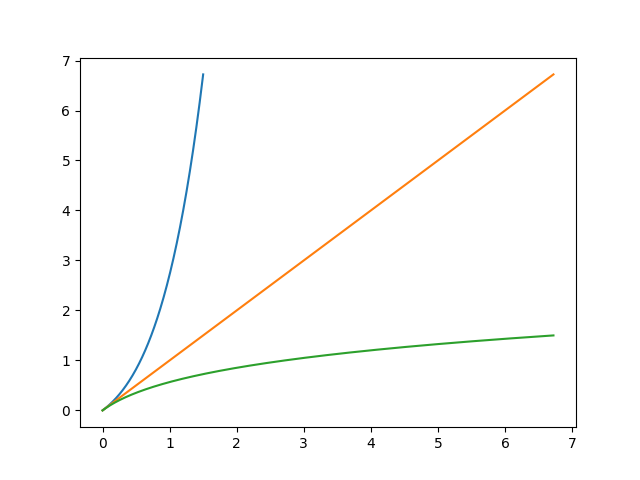
\includegraphics[scale=0.5]{graph-kholle-W.png}

\subsection{kholleur/euse: M.Thevenet}

note: 8/20 \\
chapitre: surjection, injection, bijection

\subsection{Je captais pas bien le cours encore}

Je suis tombé sur des questions de cours où il fallait utiliser l'écriture en compréhention des définitions d'injéction et surjection, et j'ai passé l'heure dessus... Pas grand chose à dire de plus mise à part que j'ai fais de la merde... \\


\subsection{kholleur/euse: M.Brunet}

note: 14/20 \\
chapitre: Calcule intégral

\subsection{Question jolie mais difficile sans aide un peu...}

montrer que $\forall (f,g) \in (R^R)^2$ de monotonie opposées, on a \\

$\frac{1}{b-a}\int_a^b f(t) dt \frac{1}{b-a}\int_a^b g(t) dt \leqslant \frac{1}{b-a}\int_a^b f(t) g(t) dt $ \\

\vspace{0.2cm}
\textbf{\large résolution:} \\

\vspace{0.1cm}
Soit $(f,g) \in (R^R)^2$ de monotonie opposées, on a \\

$\frac{1}{b-a}\int_a^b f(t) dt \frac{1}{b-a}\int_a^b g(t) dt \leqslant \frac{1}{b-a}\int_a^b f(t) g(t) dt $ \\
$\Leftrightarrow \int_a^b f(t) dt \int_a^b g(t) dt \leqslant (b-a) \int_a^b f(t) g(t) dt $ \\
$\Leftrightarrow \frac{d}{db} \left( \int_a^b f(t) dt \int_a^b g(t) dt \right) \leqslant \frac{d}{db} \left( (b-a) \int_a^b f(t) g(t) dt \right)$ \\
$\Leftrightarrow f(b) \int_a^b g(t) dt + g(b) \int_a^b f(t) dt  \leqslant (b-a) f(b)g(b)$ \\
$\Leftrightarrow \int_a^b f(b)g(t) + g(b)f(t) \leqslant (b-a) f(b)g(b)$ \hspace{0.2cm} Or $(b-a)f(b)g(b) = \int_a^b f(b)g(b) dt$ \\
$\Leftrightarrow \int_a^b f(b)g(t) + g(b)f(t) - f(b)g(b) \leqslant 0$ \\ 
$\Leftrightarrow \int_a^b f(b)(g(t) - g(b)) + g(b)(f(t) - f(b)) \leqslant 0$ \\ \\

Ce qui est vrai car si l'une est croissante et l'autre décroissante, l'intégrande sera négative

\subsection{kholleur/euse: Mme.Colin De Verdière}

note: 13/20 \\
chapitre: Calcule intégral

\subsection{Question de cours}

"formule du changement de variable dans une integale et démonstration" \\
Je ne savais pas trop ce qu'elle voulait dire, donc j'ai essayé de généraliser la technique du changement de variable. \\ \\

Soit $f: \mathbb{R} \mapsto \mathbb{R}, f \in C^0(\mathbb{R})$ On a donc \\
$\int_a^b f(x) dx$ \hspace{1cm} $\rightarrow$ \hspace{0.2cm} effections le changement de variable $\phi$, une bijection de $\mathbb{R}$ dans $\mathbb{R}$, et $\phi \in C^1(\mathbb{R})$, tq $x = \phi(u)$ et $dx = \phi'(u)du$, ainsi que le changement de borne $u = \phi^-1(x)$, d'où $a \rightarrow \phi^-1(a)$, et $b \rightarrow \phi^-1(b)$,\\
$=\int_{\phi^-1(a)}^{\phi^-1(b)} f(\phi(u)) \phi'(u) du$ \\ \\

Démonstration quasi triviale (dérivé)
\subsection{Question difficile}

calcuer $\int_0^{\frac{\pi}{2}} \frac{\sqrt{\cos x}}{\sqrt{\sin x} + \sqrt{\cos x}} dx$ \\

On montre facilement que c'est bien primitivable (continuité de  l'intégrande) \\

\hspace{1cm} $\rightarrow$ On remarque que l'on peut intégrer dans l'autre sens avec la proposition du roi, soit en changeant, le $\cos$ en $\sin$ \\

D'où $2\int_0^{\frac{\pi}{2}} \frac{\sqrt{\cos x}}{\sqrt{\sin x} + \sqrt{\cos x}} dx = \int_0^{\frac{\pi}{2}} \frac{\sqrt{\cos x} + \sqrt{\sin x}}{\sqrt{\sin x} + \sqrt{\cos x}} dx = \int_0^{\frac{\pi}{2}} 1 dx = \frac{\pi}{2}$ \\ \\
Donc $\int_0^{\frac{\pi}{2}} \frac{\sqrt{\cos x}}{\sqrt{\sin x} + \sqrt{\cos x}} dx = \frac{\pi}{4}$ 

\subsection{kholleur/euse: }

note: /20 \\
chapitre: 

\subsection{Question de cours}


\subsection{kholleur/euse: Mme.Aymard}

note: 10/20 \\
chapitre: réels et suites

\subsection{Question de cours : Caractérisation séqueltielle de la densité dans $\mathbb{R}$}

la caractérisation séquentielle de la densité dans $\mathbb{R}$, est \\ \\
Soit $A \in \mathbb{P}(\mathbb{R})$
$\forall x \in \mathbb{R}, \forall \epsilon > 0, \exists a \in A$ tq $|x-a| \leqslant \epsilon$ \\
$\Leftrightarrow \forall x \in \mathbb{R}\exists \left(u_n \right)_{n \in \mathbb{N}} \in A^{\mathbb{N}}$ tq $\lim_{n \rightarrow +\infty} = x$ \\
$\Leftrightarrow$ A est dense dans $\mathbb{R}$ \\ \\

$\#$ Démonstration: \\ \\
$\Rightarrow )$ Soit $x \in \mathbb{R}, \forall \epsilon > 0, \exists a \in A$ tq $|x-a| \leqslant \epsilon$ \\
$\hspace{1cm} \rightarrow$ posons $\epsilon = \frac{1}{n} \rightarrow_{n \rightarrow +\infty} 0$, On dispose donc de $a \in A$, posons $u_n = a$ \\
Donc $u_n \rightarrow_{n \rightarrow +\infty} x$ \\ \\

$\Leftarrow )$ Soit $x \in \mathbb{R}$ et $\left(u_n \right)_{n \in \mathbb{N}} \in \mathbb{R}$, tq $\lim_{n \rightarrow + \infty} = x$, doncc $\forall \epsilon > 0$, on dispose de $N \in \mathbb{N}$ tq $\forall n \geqslant N |x-u_n| \leqslant \epsilon$, en posant $a = u_N$, on obtient le résultat voulu \\ \\

\subsection{Exercice: étudier $u_{n+1} = \frac{1}{6} \left({u_n}^2 + 8 \right)$ }
\vspace{0.4cm}

On a une suite défini par réccurence par $u_{n+1} = f( u_n )$, avec, ici $f: x \mapsto \frac{1}{6} \left(x^2 + 8 \right)$ \\

$\hspace{1cm} \rightarrow$ étudions $f(x) - x$: déjà, $f(x) - x \geqslant 0 \Rightarrow x \geqslant 2$ sur $\mathbb{R}^+$





\begin{center}
\textbf{\large Physique}
\end{center} \vspace{0.2cm}

\section{Kholle 1}
\subsection{kholleur/euse: M.chapon ou M.Didelot}

\vspace{5mm}


\begin{center}
\textbf{\large Anglais}
\end{center} \vspace{0.2cm}

\section{Kholle 1}
\subsection{kholleur/euse: M}


\begin{center}
\textbf{\large Francais}
\end{center} \vspace{0.2cm}

\section{Kholle 1}
\subsection{kholleur/euse: Mme.}



\end{document}
